\section{Теоретическая часть}
Для данной системы определим эндогенные и экзогенные переменные.
К эндогенным переменным можно отнести:
\begin{enumerate}
	\item время обслуживания заявки i-ым оператором;
	\item время обработки запросов на j-ом компьютере.
\end{enumerate}

Экзогенная переменная - число поступивших в систему заявок.

Вероятность отказа можно рассчитать по след. формуле:

\begin{equation}
P_{\textbf{refuse} = \frac{C_{\textbf{refuse}}}{C_{\textbf{all}}}}
\end{equation}

где $P_{\textbf{refuse}}$ - вероятность отказа в обслуживании. $С_{\textbf{refuse}}$ - число заявок, которым было откзано в обслуживании, $C_{\textbf{all}}$ - общее число заявок, которое можно предтсавить в виде $C_{\textbf{all}} = C_{\textbf{served}} + C_{\textbf{refuse}}$

На рисунке \ref{fig:shema1} показана схема работы инф. центра. В данной схема S1, S2, S3 обозначают соот. операторов, а с помощью S4 и S5 - компьютеры, на которые передаются запросы от операторов.

% TODO: \usepackage{graphicx} required
\begin{figure}[h]
	\centering
	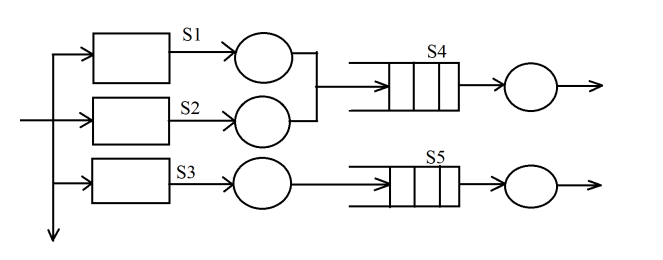
\includegraphics[width=0.7\linewidth]{shema1}
	\caption{Схема работы инф. центра}
	\label{fig:shema1}
\end{figure}
